\documentclass[12 pt,fullpage]{article}
%\documentclass[draft]{ectaart}
%%%%%%%%%%%%%%%%%%%%%%%%%%%%%%%%%%%%%%%%%%%%%%%%%%%%%%%%%%%%%%%%%%%%%%%%%%%%%%%%%%%%%%%%%%%%%%%%%%%%%%%%%%%%%%%%%%%%%%%%%%%%%%%%%%%%%%%%%%%%%%%%%%%%%%%%%%%%%%%%%%%%%%%%%%%%%%%%%%%%%%%%%%%%%%%%%%%%%%%%%%%%%%%%%%%%%%%%%%%%%%%%%%%%%%%%%%%%%%%%%%%%%%%%%%%%
\usepackage{graphicx}
\usepackage{amsfonts}
\usepackage{amssymb}
\usepackage{amsmath}
\usepackage{amsthm}
\usepackage{textcomp}
\usepackage{ifsym}
\usepackage{mathrsfs}
\usepackage{epstopdf}
\usepackage{MnSymbol}
\usepackage{multirow}
\usepackage{epsfig}
\usepackage[normalem]{ulem}
\usepackage[round]{natbib}
\usepackage{array}
\usepackage{caption}
\usepackage{subcaption}
\usepackage{url}
\usepackage{placeins}
\usepackage{longtable}
\usepackage{pdflscape}
\usepackage{tabularx}
\usepackage{booktabs}
%\usepackage{xcolor}
\usepackage{bbm}
\usepackage[colorlinks,citecolor=blue]{hyperref}
\usepackage[margin=1.1in]{geometry}
\usepackage{hyperref}
\usepackage{comment}
\usepackage{chngcntr}
\usepackage{amsmath}
\usepackage{setspace}
%\usepackage{colortbl}
\usepackage[table,xcdraw]{xcolor}

%\usepackage[bottom]{footmisc}
\usepackage[hang,flushmargin]{footmisc}
\counterwithout{equation}{section} 
%\counterwithin{equation}{chapter} 
%\numberwithin{equation}{section}

\newcommand{\footremember}[2]{%
	\footnote{#2}
	\newcounter{#1}
	\setcounter{#1}{\value{footnote}}%
}
\newcommand{\footrecall}[1]{%
	\footnotemark[\value{#1}]%
}

\setcounter{MaxMatrixCols}{10}

\linespread{1.5}



%\topmargin=-1.8cm \textheight=23.8cm \oddsidemargin=-0.3cm
%\evensidemargin=-0.5cm \textwidth=17.1cm

\DeclareMathOperator*{\argmax}{arg\,max}
\DeclareMathOperator*{\argmin}{arg\,min}
\theoremstyle{plain}
\newtheorem{theo}{Theorem}
\newtheorem{conj}{Conjecture}
\newtheorem{prop}{Proposition}
\newtheorem*{prop*}{Proposition}
\newtheorem{coro}{Corollary}
\newtheorem{lemma}{Lemma}
\newtheorem*{lemma*}{Lemma}
\newtheorem{assum}{Assumption}
\newtheorem{defi}{Definition}

\newtheorem{innercustomgeneric}{\customgenericname}
\providecommand{\customgenericname}{}
\newcommand{\newcustomtheorem}[2]{%
	\newenvironment{#1}[1]
	{%
		\renewcommand\customgenericname{#2}%
		\renewcommand\theinnercustomgeneric{##1}%
		\innercustomgeneric
	}
	{\endinnercustomgeneric}
}

\newcustomtheorem{customprop}{Proposition}
\newcustomtheorem{customlemma}{Lemma}

\def\sym#1{\ifmmode^{#1}\else\(^{#1}\)\fi}


\newcommand{\figtext}[1]{
	\vspace{-1.9ex}
	\captionsetup{justification=justified,font=footnotesize}
	\caption*{\hspace{6pt}\hangindent=1.5em #1}
}
\newcommand{\fignote}[1]{\figtext{\emph{Note:~}~#1}}

\newcommand{\figsource}[1]{\figtext{\emph{Source:~}~#1}}

\newcommand{\starnote}{\figtext{* p $<$ 0.1, ** p $<$ 0.05, *** p $<$ 0.01. Standard errors in parentheses.}}

\title{\textbf{Fentanyl Consumption and Peasants Income}}
\author{\vspace{-30mm}}

\begin{document}
	\date{\vspace{-25mm}}
	\maketitle
	\vspace{-15mm}



\newpage
%\subsection*{Preliminar regression}

\begin{table}[h!]
	\begin{center}
		\scalebox{0.6}{
			\begin{tabular}{lcccc} \\ \hline 
                    &\multicolumn{1}{c}{(1)}         &\multicolumn{1}{c}{(2)}         &\multicolumn{1}{c}{(3)}         &\multicolumn{1}{c}{(4)}         \\
 & \multicolumn{4}{c}{Income} \\ \cline{2-5} & Survey  &  \multicolumn{1}{c}{Big} & \multicolumn{1}{c}{Medium}& \multicolumn{1}{c}{Small} \\ \hline   &  &  &  &  \\ \textbf{Panel A: Full sample} \\ & & & & \\
Log Number of deaths (US) caused only by fentanyl&      -0.022         &      -0.280         &      -0.157\sym{*}  &      -0.055\sym{*}  \\
                    &     (0.061)         &     (0.437)         &     (0.067)         &     (0.024)         \\
\addlinespace
Log Number of deaths (US) caused only by cocaine&       0.172         &       1.312         &      -0.070         &      -0.050         \\
                    &     (0.096)         &     (0.881)         &     (0.119)         &     (0.044)         \\
\addlinespace
State CPI           &       0.003         &      -0.079\sym{*}  &      -0.024\sym{***}&      -0.010\sym{***}\\
                    &     (0.004)         &     (0.037)         &     (0.003)         &     (0.001)         \\
\addlinespace
Participation rate  &       0.000         &      -0.002         &       0.000         &       0.000         \\
                    &     (0.003)         &     (0.016)         &     (0.001)         &     (0.000)         \\
\addlinespace
Log Exchange rate (COP/USD)&      -0.223         &       2.786\sym{*}  &       0.561\sym{***}&       0.204\sym{***}\\
                    &     (0.126)         &     (1.270)         &     (0.085)         &     (0.032)         \\
\addlinespace
Log Estimated Coca Production based on Quinoa&      -0.012         &      -0.304         &       0.075\sym{**} &       0.031\sym{**} \\
                    &     (0.027)         &     (0.217)         &     (0.029)         &     (0.009)         \\
\addlinespace
ENSO index          &       0.013         &      -0.073         &       0.026\sym{**} &       0.008\sym{*}  \\
                    &     (0.017)         &     (0.103)         &     (0.008)         &     (0.003)         \\
\addlinespace
Economic Performance Index&       0.005         &       0.016         &       0.011\sym{***}&       0.005\sym{***}\\
                    &     (0.003)         &     (0.019)         &     (0.001)         &     (0.001)         \\
\addlinespace
COVID               &      -0.049         &      -0.400         &       0.095\sym{**} &       0.058\sym{***}\\
                    &     (0.081)         &     (0.675)         &     (0.030)         &     (0.014)         \\
\arrayrulecolor{black!10}\midrule
Observations        &         840         &         819         &         819         &         819         \\
R-squared           &       0.551         &       0.838         &       0.582         &       0.525         \\
State F.E.          &$\checkmark$         &$\checkmark$         &$\checkmark$         &$\checkmark$         \\
Month F.E.          &$\checkmark$         &$\checkmark$         &$\checkmark$         &$\checkmark$         \\


 \hline   &  &  &  &  \\ \textbf{Panel B: Sub sample from October 2014} \\ & & & & \\
Log Number of deaths (US) caused only by fentanyl&      -0.111         &      -0.785         &      -0.326\sym{***}&      -0.120\sym{***}\\
                    &     (0.101)         &     (0.904)         &     (0.065)         &     (0.024)         \\
\addlinespace
Log Number of deaths (US) caused only by cocaine&       0.127         &       2.431\sym{*}  &       0.079         &       0.018         \\
                    &     (0.110)         &     (1.081)         &     (0.112)         &     (0.042)         \\
\addlinespace
State CPI           &       0.009         &      -0.077         &      -0.013\sym{**} &      -0.005\sym{**} \\
                    &     (0.007)         &     (0.075)         &     (0.004)         &     (0.002)         \\
\addlinespace
Participation rate  &       0.003         &      -0.006         &      -0.001         &      -0.000         \\
                    &     (0.003)         &     (0.012)         &     (0.002)         &     (0.001)         \\
\addlinespace
Log Exchange rate (COP/USD)&      -0.148         &       4.010\sym{**} &       0.626\sym{***}&       0.223\sym{***}\\
                    &     (0.160)         &     (1.531)         &     (0.066)         &     (0.022)         \\
\addlinespace
Log Estimated Coca Production based on Quinoa&      -0.018         &      -0.374\sym{**} &       0.038         &       0.015\sym{*}  \\
                    &     (0.015)         &     (0.143)         &     (0.024)         &     (0.006)         \\
\addlinespace
ENSO index          &      -0.007         &      -0.179         &      -0.008         &      -0.004         \\
                    &     (0.018)         &     (0.137)         &     (0.011)         &     (0.003)         \\
\addlinespace
Economic Performance Index&       0.003         &       0.033         &       0.007\sym{**} &       0.003\sym{***}\\
                    &     (0.005)         &     (0.029)         &     (0.002)         &     (0.001)         \\
\addlinespace
COVID               &      -0.070         &      -0.196         &       0.095\sym{**} &       0.053\sym{**} \\
                    &     (0.100)         &     (0.634)         &     (0.037)         &     (0.017)         \\
\arrayrulecolor{black!10}\midrule
Observations        &         609         &         609         &         609         &         609         \\
R-squared           &       0.607         &       0.861         &       0.606         &       0.575         \\
State F.E.          &$\checkmark$         &$\checkmark$         &$\checkmark$         &$\checkmark$         \\
Month F.E.          &$\checkmark$         &$\checkmark$         &$\checkmark$         &$\checkmark$         \\
\arrayrulecolor{black}\bottomrule
\multicolumn{5}{c}{*** p$<$0.01, ** p$<$0.05, * p$<$0.1}
\end{tabular}
}
		\caption{}
	\end{center}
\end{table}
\vspace{-3mm}
\footnotesize Note: This table reports the regression of income as a function of fentanyl and cocaine related deaths in the US. Column 1 shows the dependent variable as the traditional approach using survey data for average rural household income. Columns 2-4 use satellite light intensity data, in particular column 2 establishes a classification of big villages. column 3 for medium-size villages and column 4 for small cities. All columns include state and monthly fixed effects and control by standard macroeconomic variables that affects the business cycle. Unit of observation is state x month. 


\newpage
\begin{table}[h!]
	\begin{center}
		\scalebox{0.6}{
			\begin{tabular}{lcccc} \\ \hline 
                    &\multicolumn{1}{c}{(1)}         &\multicolumn{1}{c}{(2)}         &\multicolumn{1}{c}{(3)}         &\multicolumn{1}{c}{(4)}         \\
 & \multicolumn{4}{c}{Income} \\ \cline{2-5} & Survey  &  \multicolumn{1}{c}{Big} & \multicolumn{1}{c}{Medium}& \multicolumn{1}{c}{Small} \\ \hline   &  &  &  &  \\ \textbf{Panel A: Full sample} \\ & & & & \\
Log Number of deaths (US) caused only by fentanyl&      -0.022         &      -0.280         &      -0.157\sym{*}  &      -0.055\sym{*}  \\
                    &     (0.061)         &     (0.437)         &     (0.067)         &     (0.024)         \\
\arrayrulecolor{black!10}\midrule
Observations        &         840         &         819         &         819         &         819         \\
R-squared           &       0.551         &       0.838         &       0.582         &       0.525         \\
State F.E.          &$\checkmark$         &$\checkmark$         &$\checkmark$         &$\checkmark$         \\
Month F.E.          &$\checkmark$         &$\checkmark$         &$\checkmark$         &$\checkmark$         \\


 \hline   &  &  &  &  \\ \textbf{Panel B: Sub sample from October 2014} \\ & & & & \\
Log Number of deaths (US) caused only by fentanyl&      -0.111         &      -0.785         &      -0.326\sym{***}&      -0.120\sym{***}\\
                    &     (0.101)         &     (0.904)         &     (0.065)         &     (0.024)         \\
\arrayrulecolor{black!10}\midrule
Observations        &         609         &         609         &         609         &         609         \\
R-squared           &       0.607         &       0.861         &       0.606         &       0.575         \\
State F.E.          &$\checkmark$         &$\checkmark$         &$\checkmark$         &$\checkmark$         \\
Month F.E.          &$\checkmark$         &$\checkmark$         &$\checkmark$         &$\checkmark$         \\
\arrayrulecolor{black}\bottomrule
\multicolumn{5}{c}{*** p$<$0.01, ** p$<$0.05, * p$<$0.1}
\end{tabular}
}
		\caption{}
	\end{center}
\end{table}
\vspace{-3mm}
\footnotesize Note: This table reports the regression of income as a function of fentanyl and cocaine related deaths in the US. Column 1 shows the dependent variable as the traditional approach using survey data for average rural household income. Columns 2-4 use satellite light intensity data, in particular column 2 establishes a classification of big villages. column 3 for medium-size villages and column 4 for small cities. All columns include state and monthly fixed effects and control by standard macroeconomic variables that affects the business cycle. Unit of observation is state x month. 

\newpage
\begin{table}[h!]
	\begin{center}
		\scalebox{0.6}{
			\begin{tabular}{lcccccccc} \\ \hline 
                    &\multicolumn{1}{c}{(1)}         &\multicolumn{1}{c}{(2)}         &\multicolumn{1}{c}{(3)}         &\multicolumn{1}{c}{(4)}         &\multicolumn{1}{c}{(5)}         &\multicolumn{1}{c}{(6)}         &\multicolumn{1}{c}{(7)}         &\multicolumn{1}{c}{(8)}         \\
 & \multicolumn{8}{c}{Income} \\ \cline{2-5} \cline{6-9}   & Survey  &  \multicolumn{3}{c}{Light Intensity} & Survey & \multicolumn{3}{c}{Light Intensity} \\ \cline{3-5} \cline{7-9} & GEIH & Big & Medium & Small & GEIH & Big & Medium & Small \\ \hline  & & & & &  &  &  &  \\ \textbf{Panel A: Full sample} \\ & & & & & & & & \\
Log of deaths by fentanyl&      -0.001         &      -0.446\sym{**} &      -0.174\sym{***}&      -0.064\sym{***}&      -0.022         &      -0.280         &      -0.157\sym{*}  &      -0.055\sym{*}  \\
                    &     (0.014)         &     (0.179)         &     (0.025)         &     (0.009)         &     (0.061)         &     (0.437)         &     (0.067)         &     (0.024)         \\
\addlinespace
Log of deaths by cocaine&                     &                     &                     &                     &       0.172         &       1.312         &      -0.070         &      -0.050         \\
                    &                     &                     &                     &                     &     (0.096)         &     (0.881)         &     (0.119)         &     (0.044)         \\
\addlinespace
State CPI           &                     &                     &                     &                     &       0.003         &      -0.079\sym{*}  &      -0.024\sym{***}&      -0.010\sym{***}\\
                    &                     &                     &                     &                     &     (0.004)         &     (0.037)         &     (0.003)         &     (0.001)         \\
\addlinespace
Participation rate  &                     &                     &                     &                     &       0.000         &      -0.002         &       0.000         &       0.000         \\
                    &                     &                     &                     &                     &     (0.003)         &     (0.016)         &     (0.001)         &     (0.000)         \\
\addlinespace
Log Exchange rate (COP/USD)&                     &                     &                     &                     &      -0.223         &       2.786\sym{*}  &       0.561\sym{***}&       0.204\sym{***}\\
                    &                     &                     &                     &                     &     (0.126)         &     (1.270)         &     (0.085)         &     (0.032)         \\
\addlinespace
Log Estimated Coca Production&                     &                     &                     &                     &      -0.012         &      -0.304         &       0.075\sym{**} &       0.031\sym{**} \\
                    &                     &                     &                     &                     &     (0.027)         &     (0.217)         &     (0.029)         &     (0.009)         \\
\addlinespace
ENSO index          &                     &                     &                     &                     &       0.013         &      -0.073         &       0.026\sym{**} &       0.008\sym{*}  \\
                    &                     &                     &                     &                     &     (0.017)         &     (0.103)         &     (0.008)         &     (0.003)         \\
\addlinespace
Economic Performance Index&                     &                     &                     &                     &       0.005         &       0.016         &       0.011\sym{***}&       0.005\sym{***}\\
                    &                     &                     &                     &                     &     (0.003)         &     (0.019)         &     (0.001)         &     (0.001)         \\
\addlinespace
COVID               &                     &                     &                     &                     &      -0.049         &      -0.400         &       0.095\sym{**} &       0.058\sym{***}\\
                    &                     &                     &                     &                     &     (0.081)         &     (0.675)         &     (0.030)         &     (0.014)         \\
\arrayrulecolor{black!10}\midrule
Observations        &         951         &         936         &         936         &         936         &         840         &         819         &         819         &         819         \\
R-squared           &       0.477         &       0.694         &       0.523         &       0.460         &       0.551         &       0.838         &       0.582         &       0.525         \\
State F.E.          &$\checkmark$         &$\checkmark$         &$\checkmark$         &$\checkmark$         &$\checkmark$         &$\checkmark$         &$\checkmark$         &$\checkmark$         \\
Month F.E.          &$\checkmark$         &$\checkmark$         &$\checkmark$         &$\checkmark$         &$\checkmark$         &$\checkmark$         &$\checkmark$         &$\checkmark$         \\


 \hline  & & & & &  &  &  &  \\ \textbf{Panel B: Sub sample from October 2014} \\ & & & & & & & & \\
Log of deaths by fentanyl&      -0.019         &      -1.044\sym{*}  &      -0.303\sym{***}&      -0.112\sym{***}&      -0.111         &      -0.785         &      -0.326\sym{***}&      -0.120\sym{***}\\
                    &     (0.020)         &     (0.446)         &     (0.029)         &     (0.010)         &     (0.101)         &     (0.904)         &     (0.065)         &     (0.024)         \\
\addlinespace
Log of deaths by cocaine&                     &                     &                     &                     &       0.127         &       2.431\sym{*}  &       0.079         &       0.018         \\
                    &                     &                     &                     &                     &     (0.110)         &     (1.081)         &     (0.112)         &     (0.042)         \\
\addlinespace
State CPI           &                     &                     &                     &                     &       0.009         &      -0.077         &      -0.013\sym{**} &      -0.005\sym{**} \\
                    &                     &                     &                     &                     &     (0.007)         &     (0.075)         &     (0.004)         &     (0.002)         \\
\addlinespace
Participation rate  &                     &                     &                     &                     &       0.003         &      -0.006         &      -0.001         &      -0.000         \\
                    &                     &                     &                     &                     &     (0.003)         &     (0.012)         &     (0.002)         &     (0.001)         \\
\addlinespace
Log Exchange rate (COP/USD)&                     &                     &                     &                     &      -0.148         &       4.010\sym{**} &       0.626\sym{***}&       0.223\sym{***}\\
                    &                     &                     &                     &                     &     (0.160)         &     (1.531)         &     (0.066)         &     (0.022)         \\
\addlinespace
Log Estimated Coca Production&                     &                     &                     &                     &      -0.018         &      -0.374\sym{**} &       0.038         &       0.015\sym{*}  \\
                    &                     &                     &                     &                     &     (0.015)         &     (0.143)         &     (0.024)         &     (0.006)         \\
\addlinespace
ENSO index          &                     &                     &                     &                     &      -0.007         &      -0.179         &      -0.008         &      -0.004         \\
                    &                     &                     &                     &                     &     (0.018)         &     (0.137)         &     (0.011)         &     (0.003)         \\
\addlinespace
Economic Performance Index&                     &                     &                     &                     &       0.003         &       0.033         &       0.007\sym{**} &       0.003\sym{***}\\
                    &                     &                     &                     &                     &     (0.005)         &     (0.029)         &     (0.002)         &     (0.001)         \\
\addlinespace
COVID               &                     &                     &                     &                     &      -0.070         &      -0.196         &       0.095\sym{**} &       0.053\sym{**} \\
                    &                     &                     &                     &                     &     (0.100)         &     (0.634)         &     (0.037)         &     (0.017)         \\
\arrayrulecolor{black!10}\midrule
Observations        &         690         &         696         &         696         &         696         &         609         &         609         &         609         &         609         \\
R-squared           &       0.517         &       0.721         &       0.603         &       0.567         &       0.607         &       0.861         &       0.606         &       0.575         \\
State F.E.          &$\checkmark$         &$\checkmark$         &$\checkmark$         &$\checkmark$         &$\checkmark$         &$\checkmark$         &$\checkmark$         &$\checkmark$         \\
Month F.E.          &$\checkmark$         &$\checkmark$         &$\checkmark$         &$\checkmark$         &$\checkmark$         &$\checkmark$         &$\checkmark$         &$\checkmark$         \\
\arrayrulecolor{black}\bottomrule
\multicolumn{9}{c}{*** p$<$0.01, ** p$<$0.05, * p$<$0.1. Standard errors clustered by state}
\end{tabular}
}
		\caption{}
	\end{center}
\end{table}
\vspace{-3mm}
\footnotesize Note: This table reports the regression of income as a function of fentanyl and cocaine related deaths in the US. Column 1 shows the dependent variable as the traditional approach using survey data for average rural household income. Columns 2-4 use satellite light intensity data, in particular column 2 establishes a classification of big villages. column 3 for medium-size villages and column 4 for small cities. All columns include state and monthly fixed effects and control by standard macroeconomic variables that affects the business cycle. Unit of observation is state x month. 

\newpage
\begin{table}[h!]
	\begin{center}
		\scalebox{0.6}{
			\begin{tabular}{lcccccccc} \\ \hline 
                    &\multicolumn{1}{c}{(1)}         &\multicolumn{1}{c}{(2)}         &\multicolumn{1}{c}{(3)}         &\multicolumn{1}{c}{(4)}         &\multicolumn{1}{c}{(5)}         &\multicolumn{1}{c}{(6)}         &\multicolumn{1}{c}{(7)}         &\multicolumn{1}{c}{(8)}         \\
 & \multicolumn{8}{c}{Income} \\ \cline{2-5} \cline{6-9}   & Survey  &  \multicolumn{3}{c}{Light Intensity} & Survey & \multicolumn{3}{c}{Light Intensity} \\ \cline{3-5} \cline{7-9} & GEIH & Big & Medium & Small & GEIH & Big & Medium & Small \\ \hline  & & & & &  &  &  &  \\ \textbf{Panel A: Full sample} \\ & & & & & & & & \\
Log of deaths by fentanyl&      -0.001         &      -0.446\sym{**} &      -0.174\sym{***}&      -0.064\sym{***}&      -0.022         &      -0.280         &      -0.157\sym{*}  &      -0.055\sym{*}  \\
                    &     (0.014)         &     (0.179)         &     (0.025)         &     (0.009)         &     (0.061)         &     (0.437)         &     (0.067)         &     (0.024)         \\
\addlinespace
Log of deaths by cocaine&                     &                     &                     &                     &       0.172         &       1.312         &      -0.070         &      -0.050         \\
                    &                     &                     &                     &                     &     (0.096)         &     (0.881)         &     (0.119)         &     (0.044)         \\
\addlinespace
Log Estimated Coca Production&                     &                     &                     &                     &      -0.012         &      -0.304         &       0.075\sym{**} &       0.031\sym{**} \\
                    &                     &                     &                     &                     &     (0.027)         &     (0.217)         &     (0.029)         &     (0.009)         \\
\arrayrulecolor{black!10}\midrule
Observations        &         951         &         936         &         936         &         936         &         840         &         819         &         819         &         819         \\
R-squared           &       0.477         &       0.694         &       0.523         &       0.460         &       0.551         &       0.838         &       0.582         &       0.525         \\
Controls            &    $\times$         &    $\times$         &    $\times$         &    $\times$         &$\checkmark$         &$\checkmark$         &$\checkmark$         &$\checkmark$         \\
State F.E.          &$\checkmark$         &$\checkmark$         &$\checkmark$         &$\checkmark$         &$\checkmark$         &$\checkmark$         &$\checkmark$         &$\checkmark$         \\
Month F.E.          &$\checkmark$         &$\checkmark$         &$\checkmark$         &$\checkmark$         &$\checkmark$         &$\checkmark$         &$\checkmark$         &$\checkmark$         \\


 \hline  & & & & &  &  &  &  \\ \textbf{Panel B: Sub sample} \\ & & & & & & & & \\
Log of deaths by fentanyl&      -0.019         &      -1.044\sym{*}  &      -0.303\sym{***}&      -0.112\sym{***}&      -0.111         &      -0.785         &      -0.326\sym{***}&      -0.120\sym{***}\\
                    &     (0.020)         &     (0.446)         &     (0.029)         &     (0.010)         &     (0.101)         &     (0.904)         &     (0.065)         &     (0.024)         \\
\addlinespace
Log of deaths by cocaine&                     &                     &                     &                     &       0.127         &       2.431\sym{*}  &       0.079         &       0.018         \\
                    &                     &                     &                     &                     &     (0.110)         &     (1.081)         &     (0.112)         &     (0.042)         \\
\addlinespace
Log Estimated Coca Production&                     &                     &                     &                     &      -0.018         &      -0.374\sym{**} &       0.038         &       0.015\sym{*}  \\
                    &                     &                     &                     &                     &     (0.015)         &     (0.143)         &     (0.024)         &     (0.006)         \\
\arrayrulecolor{black!10}\midrule
Observations        &         690         &         696         &         696         &         696         &         609         &         609         &         609         &         609         \\
R-squared           &       0.517         &       0.721         &       0.603         &       0.567         &       0.607         &       0.861         &       0.606         &       0.575         \\
Controls            &    $\times$         &    $\times$         &    $\times$         &    $\times$         &$\checkmark$         &$\checkmark$         &$\checkmark$         &$\checkmark$         \\
State F.E.          &$\checkmark$         &$\checkmark$         &$\checkmark$         &$\checkmark$         &$\checkmark$         &$\checkmark$         &$\checkmark$         &$\checkmark$         \\
Month F.E.          &$\checkmark$         &$\checkmark$         &$\checkmark$         &$\checkmark$         &$\checkmark$         &$\checkmark$         &$\checkmark$         &$\checkmark$         \\
\arrayrulecolor{black}\bottomrule
\end{tabular}
}
		\caption{}
	\end{center}
\end{table}
\vspace{-3mm}
\footnotesize Note: This table reports the regression of income as a function of fentanyl and cocaine related deaths in the US. Column 1 shows the dependent variable as the traditional approach using survey data for average rural household income. Columns 2-4 use satellite light intensity data, in particular column 2 establishes a classification of big villages. column 3 for medium-size villages and column 4 for small cities. All columns include state and monthly fixed effects and control by standard macroeconomic variables that affects the business cycle. Unit of observation is state x month. 

\newpage
\begin{table}[h!]
	\begin{center}
		\scalebox{0.6}{
			\begin{tabular}{lcccc} \\ \hline 
                    &\multicolumn{1}{c}{(1)}         &\multicolumn{1}{c}{(2)}         &\multicolumn{1}{c}{(3)}         &\multicolumn{1}{c}{(4)}         \\
 & \multicolumn{4}{c}{Income} \\ \cline{2-5} & Survey  &  \multicolumn{1}{c}{Big} & \multicolumn{1}{c}{Medium}& \multicolumn{1}{c}{Small} \\ \hline   &  &  &  &  \\ \textbf{Panel A: Full sample} \\ & & & & \\
Log Number of deaths (US) caused only by fentanyl&      -0.035\sym{*}  &      -0.883\sym{*}  &      -0.209\sym{***}&      -0.077\sym{***}\\
                    &     (0.017)         &     (0.389)         &     (0.028)         &     (0.010)         \\
\addlinespace
Log Number of deaths (US) caused only by cocaine&       0.259\sym{**} &       3.299         &       0.260\sym{***}&       0.100\sym{***}\\
                    &     (0.087)         &     (1.847)         &     (0.069)         &     (0.024)         \\
\arrayrulecolor{black!10}\midrule
Observations        &         951         &         936         &         936         &         936         \\
R-squared           &       0.488         &       0.698         &       0.528         &       0.465         \\
State F.E.          &$\checkmark$         &$\checkmark$         &$\checkmark$         &$\checkmark$         \\
Month F.E.          &$\checkmark$         &$\checkmark$         &$\checkmark$         &$\checkmark$         \\


 \hline   &  &  &  &  \\ \textbf{Panel B: Sub sample from October 2014} \\ & & & & \\
Log Number of deaths (US) caused only by fentanyl&      -0.042         &      -1.316\sym{*}  &      -0.313\sym{***}&      -0.116\sym{***}\\
                    &     (0.023)         &     (0.574)         &     (0.030)         &     (0.010)         \\
\addlinespace
Log Number of deaths (US) caused only by cocaine&       0.268\sym{**} &       3.252         &       0.115         &       0.044         \\
                    &     (0.103)         &     (1.731)         &     (0.081)         &     (0.033)         \\
\arrayrulecolor{black!10}\midrule
Observations        &         690         &         696         &         696         &         696         \\
R-squared           &       0.528         &       0.725         &       0.604         &       0.568         \\
State F.E.          &$\checkmark$         &$\checkmark$         &$\checkmark$         &$\checkmark$         \\
Month F.E.          &$\checkmark$         &$\checkmark$         &$\checkmark$         &$\checkmark$         \\
\arrayrulecolor{black}\bottomrule
\multicolumn{5}{c}{*** p$<$0.01, ** p$<$0.05, * p$<$0.1}
\end{tabular}
}
		\caption{}
	\end{center}
\end{table}
\vspace{-3mm}
\footnotesize Note:

\newpage
\begin{figure}[h!]
	\begin{center}
		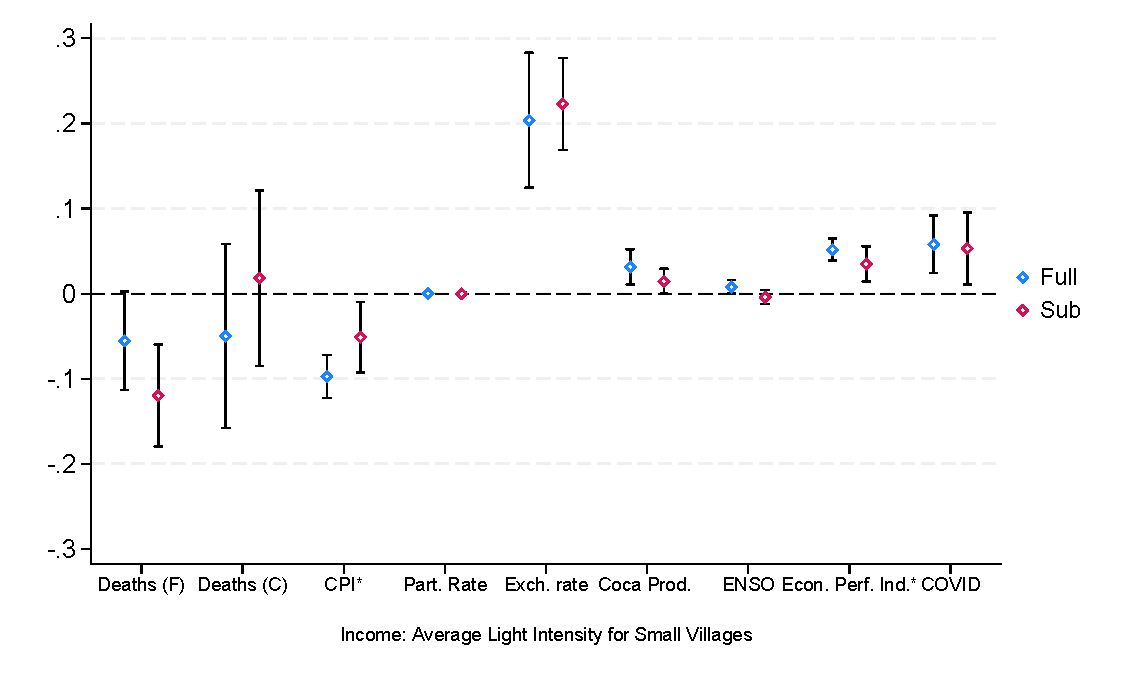
\includegraphics[width=1\textwidth]{./Figures/Figure_coef_plot.pdf}
		\caption{Coefplot}
		\label{fig:coefplot} 
	\end{center}
	{\scriptsize Note: This figure plots the coefficients of table 1 column 4.}
\end{figure}

\end{document}